\documentclass[11pt]{article}

% font
\usepackage{helvet}
\renewcommand{\familydefault}{\sfdefault}

% formato della pagina
\usepackage{geometry}
\geometry{
   a4paper,
   total={160mm,257mm},
   left=17mm,
   right=17mm,
   top=20mm,
}

% tabelle
\usepackage{tabularx}
\usepackage{ltablex}

% immagini
\usepackage{graphicx}
\usepackage{float}

\begin{document}

\begin{center}
    \huge\textbf{Title DB}
\end{center}

\section{Abstract}

\textit{\{nome-sito\}} è un azienda italiana che vuole aprire la propria attività di mercato online
sul territorio nazionale e come tale necessità di un database per la gestione delle sue risorse.\\
Grazie a \textit{\{nome-sito\}} sarà possibile fare acquisti tra una vasta serie di prodotti 
senza doversi recare in negozio, potendo scegliere se ricevere la consegna direttamente a casa
propria oppure specificando durante l'acquisto il punto di ritiro che si preferisce,
per poi andarlo a ritirare personalmente.\\
Ogni utente che desidera fare degli acquisti dovrà registrarsi attraverso la propria email,
aggiungendo i propri dati personali e i metodi di pagamento direttamente nel sito.
Inoltre per chi lo desidera ci si potrà abbonare all'offerta "Prime" per evitare i costi di spedizione
su tutti i prodotti certificati Prime e per poter ricevere le propire consegne in brevissimo tempo.
In più verrà fornito l'accesso ad altri servizi esclusivi \textit{\{nome-sito\}}.\\
Visualizzando i propri acquisti sarà possibile conoscere la data di presa in carico della spedizione
e quella di arrivo al punto di consegna. In caso di necessità sarà anche possibile specificare alcune preferenze
di spedizione, in segutio all'avvenuta operazione di acquisto dei propri prodotti.\\
\textit{\{nome-sito\}} assicura ai propri clienti che i fornitori siano accertati mettendo a disposizione
la località di produzione ed un recapito telefonico.\\
In caso di guasto o per via di una determinata motivazione specificata dall'utente sarà
possibile effettuare il reso dei prodotti acquistati avendo la garanzia di rimborso della spesa. 

\section{Analisi dei requisiti}

\subsection{Descrizione testuale}

Nella base di dati sono presenti i dati degli \textbf{utenti} registrati, di ogni utente sono noti:
\begin{itemize}
    \item Nome
    \item Cognome
    \item Indirizzo email
    \item Password 
    \item Numero di telefono
    \item Indirizzo di residenza per la consegna
    \item Metodi di pagamento
\end{itemize}
Un utente può abbonarsi all'offerta "Prime", che avrà durata mensile o annuale in base alla scelta dell'utente.
L'utente abbonato non paga i costi di spedizione su tutti i prodotti indicati.\\
Le \textbf{carte di credito} utilizzate dall’utente devono essere provviste di:
\begin{itemize}
    \item Numero
    \item Circuito (Mastercard, Visa, …)
    \item Scadenza
    \item CVV
    \item Intestatario
\end{itemize}
I pagamenti vengono autorizzati attraverso un sito esterno, rilevato automaticamente dal circuito.\\
Ogni \textbf{fornitore} deve fornire le informazioni riguardo a:
\begin{itemize}
    \item Nome
    \item Numero di telefono
    \item Indirizzo email
    \item Partita IVA
    \item Indirizzo (Via, Numero civico, CAP, Città, Provincia, Stato) dei propri stabilimenti
\end{itemize} 
Gli stabilimenti dei fornitori possono trovarsi anche in paesi esteri fuori dall'Italia.\\
Di ogni \textbf{prodotto}, si vuole conoscere:
\begin{itemize}
    \item Codice
    \item Nome
    \item Prezzo
    \item Quantità disponibile
    \item Peso
    \item Descrizione
    \item Costo di spedizione
    \item Offerta prime
\end{itemize}
Ogni \textbf{ordine} deve memorizzare le informazioni riguardo:
\begin{itemize}
    \item Carrello (Utente e Prodotti ordinati)
    \item Metodo di pagamento utilizzato
    \item Data e ora di acquisto
    \item Importo pagato
    \item Indirizzo di consegna
    \item Preferenze di spedizione (opzionale)
\end{itemize}
Gli ordini possono essere ritirati dal cliente, in quel caso deve essergli fornita la data e l’ora di arrivo della propria consegna al punto di ritiro
scelto oppure possono essere spediti all'indirizzo di residenza dell'utente.\\
Quando viene richiesta una \textbf{spedizione} si vogliono memorizzare le informazioni riguardo:
\begin{itemize}
    \item Codice
    \item Data di partenza prevista
    \item Data di arrivo prevista
    \item Data effettiva
\end{itemize}
Per ricevere i propri prodotti interessa conoscere i \textbf{punti di consegna}. Per ogni Punto di consegna si vogliono
memorizzare le seguenti informazioni:
\begin{itemize}
    \item Indirizzo (Via, Numero civico, CAP, Città, Provincia, Stato)
\end{itemize}
Inoltre, se il punto di consegna è un punto di ritiro scelto dall'utente (e quindi non il suo indirizzo di residenza), ci interessa sapere:
\begin{itemize}
    \item Orario di apertura
    \item Orario di chiusura
\end{itemize}
Infine per effettuare un \textbf{reso} è necessario specificare:
\begin{itemize}
    \item Utente
    \item Prodotto acquistato
    \item Quantità da rendere
    \item Motivazione 
\end{itemize}

\subsection{Glossario dei termini}

\begin{center}
    
    \begin{tabularx}{0.99\textwidth} {
        | >{\raggedright\arraybackslash}>{\hsize=.3\hsize}X |
          >{\raggedright\arraybackslash}                  X |
          >{\raggedright\arraybackslash}>{\hsize=.5\hsize}X |
    }
        \hline
        \textbf{Termine} & \textbf{Descrizione} & \textbf{Collegamenti} \\
        \hline\hline

        %Termine
        Utente &
        %Descrizione
        Utente registrato al sito &
        %Collegamenti
        Carrello, CartaDiCredito, Residenza \\ 
        \hline

        %Termine
        Prime &
        %Descrizione
        Utente dotato di un abbonamento attivo che usufruisce delle agevolazioni di acquisto e spedizione &
        %Collegamenti
        Entità figlia di Utente \\ 
        \hline

        %Termine
        Carrello &
        %Descrizione
        Zona di memorizzazione dei prodotti selezionati che non sono ancora stati acquistati  &
        %Collegamenti
        Prodotto, Ordine, Utente\\
        \hline

        %Termine
        Prodotto &
        %Descrizione
        Un bene tangibile, venduto nel sito e acquistabile da qualunque utente &
        %Collegamenti
        Fornitore, Carrello, Reso\\
        \hline

        %Termine
        Costo spedizione &
        %Descrizione
        Il costo della spedizione (nel caso di validità "Prime" questo non viene calcolato nell'importo totale) &
        %Collegamenti
        Attributo di Prodotto\\
        \hline

        %Termine
        Importo &
        %Descrizione
        Costo totale relativo ad un ordine. Ogni prodotto comprende anche i costi di spedizione &
        %Collegamenti
        Attributo di Ordine \\ 
        \hline

        %Termine
        Fornitore &
        %Descrizione
        L'ente che produce e mette in vendita i propri prodotti &
        %Collegamenti
        Prodotto, Stabilimento \\ 
        \hline  

        %Termine
        PIVA &
        %Descrizione
        La partita IVA è una sequenza di cifre che identifica univocamente un soggetto che esercita un'attività &
        %Collegamenti
        Attributo di Fornitore \\ 
        \hline

        %Termine
        Stabilimento &
        %Descrizione
        Una sede di produzione di un fornitore &
        %Collegamenti
        Fornitore, Reso \\ 
        \hline
        
        %Termine
        Spedizione &
        %Descrizione
        Tempo che trascorre tra la presa in carico fino al punto di consegna di uno o più ordini &
        %Collegamenti
        Ordine \\ 
        \hline

        %Termine
        Codice &
        %Descrizione
        Codice univoco dal quale è possibile ottenere le date di spedizione del proprio ordine &
        %Collegamenti
        Attributo di Spedizione \\ 
        \hline

        %Termine
        PuntoDiConsegna &
        %Descrizione
        Indirizzo di spedizione &
        %Collegamenti
        Ordine \\ 
        \hline

        %Termine
        PuntoDiRitiro &
        %Descrizione
        Esercente che fornisce il proprio stabilimento per la ricezione e il ritiro delle consegne a determinati orari &
        %Collegamenti
        Entità figlia di PuntoDiConsegna \\ 
        \hline

        %Termine
        Reso &
        %Descrizione
        La possibilità di ottenere il rimborso su un prodotto acquistato  restituendolo al fornitore &
        %Collegamenti
        Ordine, Prodotto, Stabilimento \\ 
        \hline

    \end{tabularx}
\end{center}

\subsection{Operazioni}


\begin{center}
    
    \begin{tabularx}{0.98\textwidth} {
        | >{\raggedright\arraybackslash}X |
          >{\raggedright\arraybackslash}X |
          >{\raggedright\arraybackslash}X |
    }

    \hline
    \textbf{Operazione} & \textbf{Tipo} & \textbf{Frequenza} \\
    \hline\hline

    %Operazione
    Inserimento di un nuovo utente &
    %Tipo
    S &
    %Frequenza
    500 al giorno \\
    \hline

    %Operazione
    Inserimento di un nuovo prodotto &
    %Tipo
    S &
    %Frequenza
    1000 al mese \\
    \hline

    %Operazione
    Inserimento di un nuovo ordine &
    %Tipo
    S &
    %Frequenza
    20000 al giorno \\
    \hline

    %Operazione
    Ricerca di un prodotto &
    %Tipo
    L &
    %Frequenza
    5000 all'ora \\
    \hline

    %Operazione
    Ricerca dei dati riguardanti un fornitore &
    %Tipo
    L &
    %Frequenza
    200 al giorno \\
    \hline

    %Operazione
    Visualizzazione dei prodotti nel proprio carrello &
    %Tipo
    L &
    %Frequenza
    10000 al giorno \\
    \hline

    %Operazione
    Aggiornarmento della quantità disponibile di un prodotto &
    %Tipo
    S &
    %Frequenza
    1000 al mese \\
    \hline

    %Operazione
    Richiesta di reso di un prodotto  &
    %Tipo
    S &
    %Frequenza
    2000 al mese \\
    \hline

    %Operazione
    Visualizzazione della data di arrivo del proprio ordine &
    %Tipo
    L &
    %Frequenza
    500 al giorno \\
    \hline

    %Operazione
    Ricerca della fascia oraria di apertura di un punto di ritiro &
    %Tipo
    L &
    %Frequenza
    500 al giorno \\
    \hline
    
    \end{tabularx}
\end{center}

\section{Progettazione Concettuale}

\subsection{Lista entità}

\textbf{Se non specificato l'attributo è NOT NULL}
\begin{itemize}
    \item Utente
    \begin{itemize}
        \item \underline{Email}: varchar(100) PRIMARY KEY
        \item Nome: varchar(50)
        \item Cognome: varchar(50)
        \item NumeroTelefono: varchar(15)
        \item Password: varchar(20)
        \begin{description}
            \item L'entità utente si specializza in una sottocategoria con una \textbf{generalizzazione parziale}:
        \end{description}
        \item[•] Utente Prime
        \begin{itemize}
            \item[–] DataIscrizione: timestamp
            \item[–] DataScadenza: timestamp, (\textgreater{} DataIscrizione)
            \item[–] Abbonamento: Enumerated, ("MENSILE", "ANNUALE")
        \end{itemize}
    \end{itemize}
    \item Carrello
    \begin{itemize}
        \item \underline{Id}: integer PRIMARY KEY
        \item \underline{Utente}: varchar(100) PRIMARY KEY
    \end{itemize}
    \item Prodotto
    \begin{itemize}
        \item \underline{Codice}: varchar(14) PRIMARY KEY
        \item Nome: varchar(100)
        \item Prezzo: decimal, (\textgreater{}= 0)
        \item QuantitàDisponibile: integer, (\textgreater{}= 0)
        \item Peso: decimal, (\textgreater{} 0)
        \item Descrizione: varchar(5000)
        \item CostoSpedizione: decimal, (\textgreater{}= 0)
        \item Prime: boolean
    \end{itemize}
    \item Fornitore
    \begin{itemize}
        \item \underline{PIVA}: varchar(11) PRIMARY KEY
        \item Nome: varchar(50)
        \item Email: varchar(100)
        \item NumeroTelefono: varchar(15)
    \end{itemize}
    \item Stabilimento
    \begin{itemize}
        \item \underline{Via}: varchar(100) PRIMARY KEY
        \item \underline{NumeroCivico}: varchar(10) PRIMARY KEY
        \item \underline{CAP}: varchar(5) PRIMARY KEY
        \item \underline{Città}: varchar(100)
        \item Stato: varchar(100)
    \end{itemize}
    \item CartaDiCredito
    \begin{itemize}
        \item \underline{Numero}: varchar(16) PRIMARY KEY
        \item Circuito: varchar(25)
        \item Scadenza: date
        \item CVV: varchar(3)
        \item Intestatario: varchar(50)
    \end{itemize}
    \item Ordine
    \begin{itemize}
        \item \underline{Id}: integer PRIMARY KEY
        \item \underline{Carrello}: integer PRIMARY KEY
        \item \underline{Utente}: varchar(100) PRIMARY KEY
        \item DataAcquisto: timestamp
        \item Importo: decimal
        \item PreferenzeSpedizione: varchar(500) può essere NULL
    \end{itemize}
    \item Spedizione:
    \begin{itemize}
        \item \underline{Codice}: varchar(13) PRIMARY KEY
        \item DataPartenza: timestamp
        \item DataArrivo: timestamp (\textgreater{} DataPartenza)
        \item DataEffettiva: timestamp può essere NULL
    \end{itemize}
    \item PuntoDiConsegna
    \begin{itemize}
        \item \underline{Via}: varchar(100) PRIMARY KEY
        \item \underline{NumeroCivico}: varchar(10) PRIMARY KEY
        \item \underline{CAP}: varchar(5) PRIMARY KEY
        \item \underline{Città}: varchar(100)
        \begin{description}
            \item L'entità Punto di consegna si specializza in due sottocategorie con una \textbf{generalizzazione totale}:
        \end{description}
        \item[•] PuntoDiRitiro
        \begin{itemize}
            \item[–] OraApertura: time
            \item[–] OraChiusura: time, (\textgreater{} OraApertura)
        \end{itemize}
        \item[•] Residenza
    \end{itemize}
    \item Reso
    \begin{itemize}
        \item \underline{Utente}: varchar(100) PRIMARY KEY
        \item \underline{Carrello}: integer PRIMARY KEY
        \item \underline{Ordine}: integer PRIMARY KEY
        \item \underline{Prodotto}: varchar(14) PRIMARY KEY
        \item Quantità: integer, (\textgreater{} 0)
        \item Motivazione: varchar(500)
    \end{itemize}
\end{itemize}

\subsection{Tabella delle relazioni}

\begin{center}
    \begin{tabularx}{0.98\textwidth} {
        | >{\raggedright\arraybackslash}>{\hsize=.4\hsize}X |
          >{\raggedright\arraybackslash}>{\hsize=.4\hsize}X |
          >{\raggedright\arraybackslash}                  X |
          >{\raggedright\arraybackslash}>{\hsize=.4\hsize}X |
    }
        \hline
        \textbf{Relazione} & \textbf{Entità coinvolte} & \textbf{Descrizione} & \textbf{Attributi} \\
        \hline\hline

        %Relazione
        Acquisto &
        %Entità coinvolte
        Carrello (0,1)
        Ordine (1,1) &
        %Descrizione
        Un utente può decidere di acquistare i prodotti che ha all'interno del carrello (facendo quindi un ordine relativo a quel carrello), oppure no e quindi non procedere all'acquisto &
        %Attributi
        Data e ora: TIMESTAMP \\ 
        \hline

        %Relazione
        Cliente &
        %Entità coinvolte
        Ordine (0,N)
        Reso (1,1) &
        %Descrizione
        Un utente può decidere di effettuare il reso di uno o più prodotti, in tal caso l'ordine permette di risalire al cliente che ha acquistato il prodotto da restituire  &
        %Attributi
        Nessuno \\ 
        \hline
        
        %Relazione
        Attività &
        %Entità coinvolte
        Fornitore (1,N)
        Prodotto (1,1) &
        %Descrizione
        Un fornitore può mettere in vendita un certo quantitativo di prodotti che quindi saranno riconducibili a lui  &
        %Attributi
        Nessuno \\ 
        \hline
        
        %Relazione
        Consegna &
        %Entità coinvolte
        Ordine (1,1)
        Spedizione (1,N) &
        %Descrizione
        Una volta effettuato un ordine, va organizzata una spedizione affinché venga consegnato all'utente  &
        %Attributi
        Nessuno \\ 
        \hline
        
        %Relazione
        Località &
        %Entità coinvolte
        Fornitore (1,N)
        Stabilimento (1,1) &
        %Descrizione
        Un fornitore avrà a disposizione uno o più stabilimenti che metteranno a disposizione i prodotti pronti per la vendita  &
        %Attributi
        Nessuno \\ 
        \hline
        
        %Relazione
        Località &
        %Entità coinvolte
        Residenza (1,N)
        Utente (0,1) &
        %Descrizione
        Un utente può registrare al più un indirizzo per la residenza a cui potrà far arrivare le spedizioni richieste  &
        %Attributi
        Nessuno \\ 
        \hline
        
        %Relazione
        Metodo di pagamento &
        %Entità coinvolte
        CartaDiCredito (1,1)
        Utente (1,N) &
        %Descrizione
        Un utente deve registrare uno o più metodi di pagamento, per poter effettuare degli acquisti  &
        %Attributi
        Nessuno \\ 
        \hline
        
        %Relazione
        Possiede &
        %Entità coinvolte
        Carrello (1,1)
        Utente (1,1) &
        %Descrizione
        Un utente avrà a disposizione un carrello in cui mettere tutti i prodotti che intende acquistare  &
        %Attributi
        Nessuno \\ 
        \hline
        
        %Relazione
        Prodotti salvati &
        %Entità coinvolte
        Carrello (0,N)
        Prodotto (1,1) &
        %Descrizione
        Un carrello al suo interno avrà una lista di prodotti che l'utente intende acquistare &
        %Attributi
        Quantità: INT \textgreater{} 0 \\ 
        \hline
        
        %Relazione
        Rifiuto &
        %Entità coinvolte
        Prodotto (0,N)
        Reso (1,1) &
        %Descrizione
        E' possibile effettuare il reso del prodotto se, ad esempio, non rispetta la descrizione con cui è stato presentato &
        %Attributi
        Nessuno \\ 
        \hline
        
        %Relazione
        Transazione &
        %Entità coinvolte
        CartaDiCredito (0,N)
        Ordine (1,1) &
        %Descrizione
        Una carta di credito può essere utilizzata per zero o più ordini, un ordine è sempre associato ad un metodo di pagamento &
        %Attributi
        Codice transazione: VARCHAR \\ 
        \hline
        
        %Relazione
        Trasporto &
        %Entità coinvolte
        Reso (1,1)
        Stabilimento (0,N) &
        %Descrizione
        Un prodotto che viene restituito va riportato in uno stabilimento che lo prenderà in gestione per smaltirlo &
        %Attributi
        Nessuno \\ 
        \hline
        
        %Relazione
        Trasporto &
        %Entità coinvolte
        Ordine (1,1)
        PuntoDiConsegna (0,N) &
        %Descrizione
        Una volta effettuato l'ordine, esso va consegnato all'indirizzo scelto dall'utente o, alternativamente, ad un punto di ritiro &
        %Attributi
        Nessuno \\ 
        \hline

    \end{tabularx}
\end{center}

\textbf{Vincoli non rappresentabili tramite schema E-R:}
\begin{itemize}
    \item Un cliente può effettuare il reso solo dei prodotti che ha precedentemente acquistato e che gli sono stati consegnati
    \item L'attributo importo dell'entità ordine è uguale alla somma dei prezzi dei prodotti presenti nel carrello più le relative spese di spedizione dei singoli prodotti
\end{itemize}

\textbf{Vincoli di derivazione:}
\begin{itemize}
    \item Il valore degli attributi DataIscrizione e DataScadenza dell'entità utente prime devono essere coerenti con il tipo di abbonamento dell'utente
\end{itemize}

\begin{center}
    \textbf{Schema Concettuale}
\end{center}

\begin{figure}[H]
    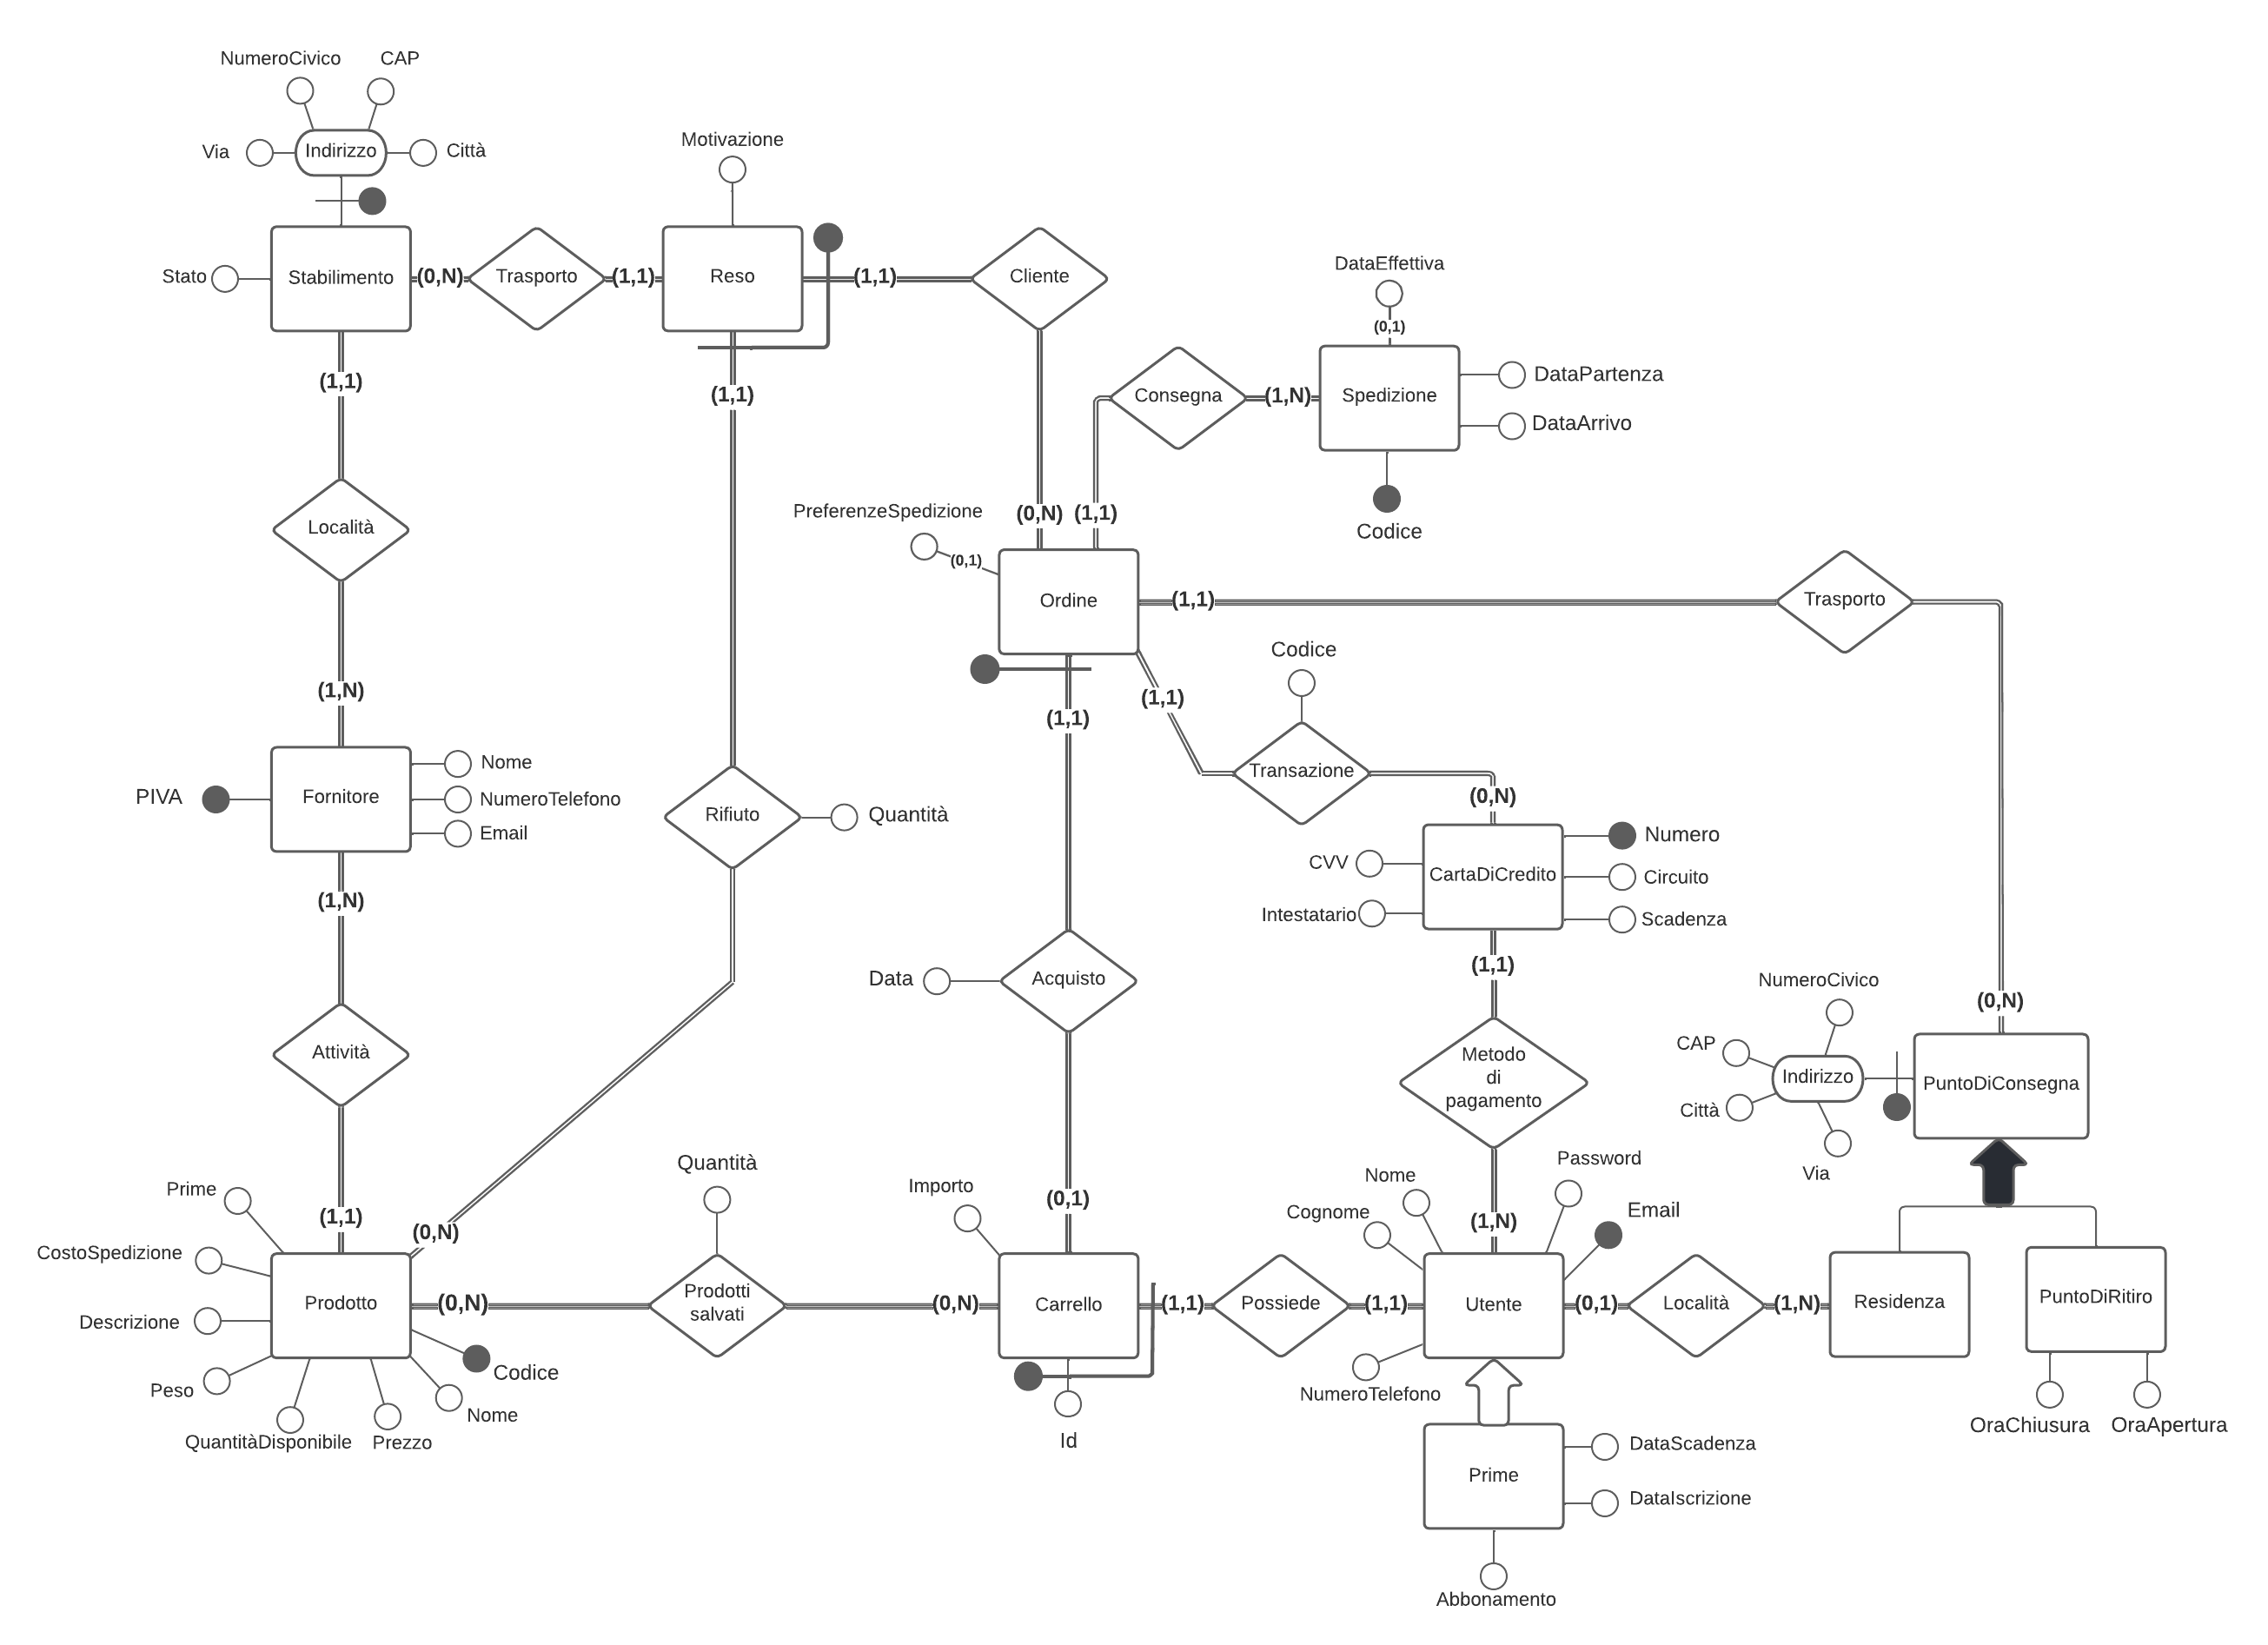
\includegraphics[scale=0.44]{media/SampleAmazonDB.png}
    \label{Schema E-R}
\end{figure}

\section{Progettazione Logica}

\subsection{Ristrutturazione}

\subsubsection{Ananlisi delle rindondanze}

\dots

\subsubsection{Eliminazione delle generalizzazioni}

\begin{center}
    \begin{tabularx}{0.97\textwidth} {
        | >{\raggedright\arraybackslash}>{\hsize=.4\hsize}X |
          >{\raggedright\arraybackslash}>{\hsize=.6\hsize}X |
        }
    
        \hline
        \textbf{Generalizzazione} & \textbf{Risoluzione} \\
        \hline\hline

        %Generalizzazione
        Utente \textless{}--- Prime &
        %Risoluzione
        L'entità Prime viene accorpata in Utente, \\
        \hline

        %Generalizzazione
        PuntoDiConsegna \textless{}--- Residenza, PuntoDiRitiro &
        %Risoluzione
        Le entità Residenza e PuntoDiRitiro ereditano l'attributo composto Indirizzo da PuntoDiConsegna.
        Perciò si rimuove l'entità padre e vengono create due nuove relazioni di Trasporto tra Ordine con
        Residenza e PuntoDiRitiro  \\
        \hline

    \end{tabularx}
\end{center}

\subsubsection{Scelta degli identificatori primari}

\dots

\subsection{Crezione delle tabelle}

\end{document}